% Chinese translation assembled from source/blocks.json.

% See source/translation.py for the translation and source/build_tex.py for assembly.

% source-block: 271211a5-58b7-808d-8b12-d403fd15edda (page; source-index: 0)

% source-block: 271211a5-58b7-8008-b8dd-de0e17512f6c (image; source-index: 1)

\begin{figure}[H]
\centering
% source-block: 271211a5-58b7-8008-b8dd-de0e17512f6c (image)

\includegraphics[width=\linewidth,height=0.64\textheight,keepaspectratio]{figures/image-00.png}
\end{figure}


% source-block: 271211a5-58b7-807e-b753-eb1f02c391cf (quote; source-index: 2)

\textbf{作者：}\href{https://www.jiacailiu.cn/}{Jiacai Liu}$^{*}$、\href{https://richardli.xyz/}{Yingru Li}$^{*\dagger}$、Yuqian Fu、Jiawei Wang、Qian Liu、Yu Shen$^{\dagger}$。


% source-block: 279211a5-58b7-807a-8502-e46110d8b45a (text; source-index: 3)

本工作在字节跳动完成。首次发表于 2025 年 9 月 17 日。


% source-block: 278211a5-58b7-80cc-846e-ff4bfb6f96fd (text; source-index: 4)

$^{*}$共同第一作者。$^{\dagger}$通讯作者。


% source-block: 311211a5-58b7-80de-b4e5-eb28c7fe3f45 (text; source-index: 5)

原文关联论文：\href{https://arxiv.org/abs/2512.23075}{Trust Region Masking for Long-Horizon LLM Reinforcement Learning（面向长时域大语言模型强化学习的信赖域掩码）}。


% source-block: 271211a5-58b7-8065-b6d3-d50fe9986453 (image; source-index: 6)

\begin{figure}[H]
\centering
% source-block: 271211a5-58b7-8065-b6d3-d50fe9986453 (image)
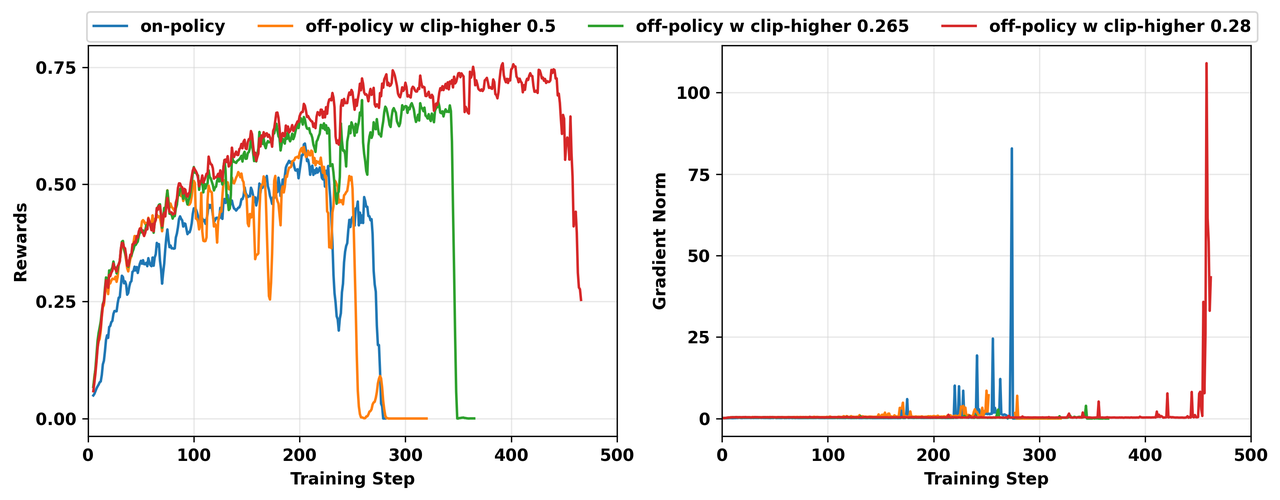
\includegraphics[width=\linewidth,height=0.64\textheight,keepaspectratio]{figures/image-01.png}
\caption*{\textbf{图 1。}Qwen3-14B-Base 上四次失败 GRPO TIR 实验的奖励（左）与梯度范数（右）。每个训练步均采样 1024 条轨迹（64 个提示 $\times$ 16 个响应），学习率为 $10^{-6}$。同策略与异策略实验的 \code{ppo_mini_batch_size} 分别为 1024 和 256。}
\end{figure}


% source-block: 291211a5-58b7-800e-b8b9-e7fec9a257a1 (callout; source-index: 7)

% source-block: 292211a5-58b7-80cb-b26d-f4398b15bb05 (text; source-index: 8)

\textbf{最新动态}（保留原文所列月日）


% source-block: 2bf211a5-58b7-80c8-a86a-d06945718bbc (text; source-index: 9)

\textbf{[12 月 2 日]} \href{https://arxiv.org/abs/2512.02556}{DeepSeek-V3.2} 采用了我们的\textbf{几何序列掩码}，用于处理训练与推理不匹配，以及一般异策略训练中的不稳定性。


% source-block: 2c3211a5-58b7-80da-a760-f6cdaa0f0c16 (text; source-index: 10)

\textbf{[12 月 1 日]} Qwen 团队在\href{https://arxiv.org/abs/2512.01374}{《稳定大语言模型强化学习：形式化与实践》}中讨论了我们的工作。


% source-block: 2a4211a5-58b7-80dd-85eb-facea672bd7c (text; source-index: 11)

\textbf{[11 月 12 日]} 面向一般异策略问题的 rollout 修正已合并至 VeRL：\href{https://verl.readthedocs.io/en/latest/algo/rollout_corr.html}{使用文档}、\href{https://verl.readthedocs.io/en/latest/algo/rollout_corr_math.html}{数学细节}。（\href{https://richardli.xyz/}{Yingru Li}）


% source-block: 2c1211a5-58b7-8048-9a1c-f48f0552fe53 (text; source-index: 12)

\textbf{[11 月 10 日]} 很高兴看到 \href{https://blog.vllm.ai/2025/11/10/bitwise-consistent-train-inference.html}{vLLM 博客}讨论了我们的工作，并实现了“逐比特一致的同策略强化学习”。


% source-block: 29d211a5-58b7-80a4-80bf-f01d038e7f08 (text; source-index: 13)

\textbf{[10 月 31 日]} VeRL 的全异步模块通过\href{https://github.com/volcengine/verl/pull/3955}{此 PR}集成了我们的工作。


% source-block: 29d211a5-58b7-8085-9333-d4ea9b6bca4f (text; source-index: 14)

\textbf{[10 月 20 日]} Slime 通过\href{https://github.com/THUDM/slime/pull/429}{此 PR}集成了我们的工作。（SGLang RL：\href{https://github.com/zhaochenyang20}{Chenyang Zhao}、\href{https://www.linkedin.com/in/jiajun-li-guapisolo/}{Jiajun Li}）


% source-block: 2c1211a5-58b7-807d-98df-e396b392553d (text; source-index: 15)

\textbf{[10 月 16 日]} 很高兴看到 Cognition 的 \href{https://cognition.ai/blog/swe-grep#motivation}{SWE-grep} 引用了我们的工作；它同样使用序列级掩码重要性采样（MIS）来处理训练与推理不匹配。


% source-block: 291211a5-58b7-80f1-9c73-f71a294cfc7d (text; source-index: 16)

\textbf{[10 月 15 日]} 一个 Megatron 训练崩溃问题通过几何级掩码得到解决。


% source-block: 291211a5-58b7-808d-870f-fcff431f4357 (external_object_instance; source-index: 17)

\href{https://github.com/volcengine/verl/issues/3597}{VeRL issue \#3597：使用 Qwen3-14B/Qwen3-30B-A3B 长时间运行 DAPO 时的 Megatron 训练崩溃。}


% source-block: 29d211a5-58b7-8053-bb32-c3122176e17b (text; source-index: 18)

\textbf{[10 月 13 日]} \href{https://github.com/volcengine/verl/releases/tag/v0.6.0}{VeRL 0.6.0} 已通过\href{https://github.com/volcengine/verl/pull/3694}{此 PR}集成我们的工作，包括新引入的\textbf{基于重要性权重几何平均值的序列掩码／拒绝方法（Geo-MIS/Geo-RS）}。（\href{https://richardli.xyz/}{Yingru Li}）


% source-block: 271211a5-58b7-80f7-8789-fd2833260f55 (callout; source-index: 19)

% source-block: 271211a5-58b7-808c-8d7b-caebe4c40799 (header; source-index: 20)

\hypertarget{src-271211a5-58b7-808c-8d7b-caebe4c40799}{}
\section*{内容提要}
\phantomsection
\addcontentsline{toc}{section}{内容提要}


% source-block: 277211a5-58b7-80a6-8d32-e5e211878239 (text; source-index: 21)

对推理速度的不懈追求，造成了危险的“训练与推理不匹配”，它可能悄无声息地破坏大语言模型强化学习。我们的研究揭示了一个恶性循环，在现代推理强化学习和智能体强化学习中尤为突出：


% source-block: 277211a5-58b7-804e-a899-cfa16040f0c7 (bulleted_list; source-index: 22)

\begin{itemize}

\item \textbf{分布外上下文促使模型采样低概率词元。}智能体工作流让模型接触外部输入和动态环境，使其频繁生成低概率词元；这些词元又是新颖推理、工具调用和适应性响应所必需的。（见\hyperlink{src-271211a5-58b7-8050-b3b1-dbbad2a1eb40}{第 3.4 节}。）

% source-block: 277211a5-58b7-80d9-ad38-ccdc1dfe9f5a (bulleted_list; source-index: 23)

\item \textbf{低概率词元加剧训练崩溃。}这些词元成为最薄弱的环节：训练与推理之间的不匹配在它们身上最为严重，会产生灾难性的大梯度，导致性能在无明显征兆的情况下下降，并突然训练失败。（见\hyperlink{src-271211a5-58b7-8043-9a6b-f4222291f060}{第 3.3 节}。）

% source-block: 277211a5-58b7-807d-900e-f24aa1b5c3f7 (bulleted_list; source-index: 24)

\item \textbf{硬件差异使问题更加复杂。}不同 GPU 架构可能以难以预测的方式加剧不匹配，因此同一套智能体训练配置可能在一台机器上成功，却在另一台机器上灾难性失败。（见\hyperlink{src-271211a5-58b7-80c9-ad90-f8aa1353bfe1}{第 3.5 节}。）

% source-block: 277211a5-58b7-8012-83a7-dd70b7fc9829 (bulleted_list; source-index: 25)

\item \textbf{序列级修正是有理论依据的解决方案。}序列级修正考虑完整的状态轨迹，修正有偏梯度，从而在不同硬件和复杂任务中恢复训练稳定性。（见\hyperlink{src-27b211a5-58b7-8099-ba48-fa8849ab54c8}{第 4.2.1 节}。）

\end{itemize}

% source-block: 2bd211a5-58b7-8033-a485-d9407b771feb (callout; source-index: 26)

% source-block: 2bd211a5-58b7-80b4-974c-c6987ef77b41 (header; source-index: 27)

\hypertarget{src-2bd211a5-58b7-80b4-974c-c6987ef77b41}{}
\section*{深入分析}
\phantomsection
\addcontentsline{toc}{section}{深入分析}


% source-block: 2bd211a5-58b7-808e-a28e-e287fc3822af (text; source-index: 28)

为更严格地剖析这一问题，我们还发表了由三篇博客构成的系列文章：


% source-block: 2c4211a5-58b7-802b-808c-f610d4db1d04 (bulleted_list; source-index: 29)

\begin{itemize}

\item \href{https://richardli.xyz/rl-collapse-1}{\textbf{第一篇：为什么异策略会破坏强化学习——SGA 分析框架。}}已有认识（TRPO 理论）：代理目标 $L_\mu(\pi)$ 是强化学习目标 $J(\pi)$ 的一阶泰勒近似；TRPO 下界 $J(\pi)\ge L_\mu(\pi)-C\cdot T^2\cdot D_{\mathrm{TV}}^{\max}$ 表明近似误差随 $T^2$ 增长，要求信赖域按 $\delta\propto 1/T^2$ 缩小。我们的见解是：词元级重要性采样（PPO/GRPO）计算的是 $\nabla L_\mu$，而非 $\nabla J$；它修正词元分布，却没有修正状态分布的不匹配（$d_\mu\ne d_\pi$），从而产生 $O(T^2D_{\mathrm{TV}}^{\max})$ 的偏差。我们通过 SGA 引理形式化了两种失效模式：由 $D_{\mathrm{TV}}$ 衡量的\textbf{偏差}，以及由 $\chi^2$ 散度衡量的\textbf{方差}；这两类指标不能互换。

% source-block: 2c4211a5-58b7-8030-bd63-d60722697c06 (bulleted_list; source-index: 30)

\item \href{https://richardli.xyz/rl-collapse-2}{\textbf{第二篇：应用 SGA 框架——词元级与序列级修正。}}我们的分析表明，词元级重要性采样（PPO/GRPO）因代理目标的一阶近似误差而具有 $O(T^2D_{\mathrm{TV}}^{\max})$ 的偏差；序列级重要性采样无偏，但具有指数级方差 $O((1+\bar{\chi}_{\max}^{\,2})^T)$。我们的方案是通过截断 $\rho(y)\to\min(\rho(y),C)$，使 Seq-TIS 获得可控的偏差与方差折中。核心结论是：这种偏差属于序列级问题，在不可忽略时需要序列级解决方案。

% source-block: 2c4211a5-58b7-8082-8edd-c06110f99479 (bulleted_list; source-index: 31)

\item \href{https://richardli.xyz/rl-collapse-3}{\textbf{第三篇：通过序列掩码实现信赖域优化。}}已有认识（TRPO 理论）：信赖域约束保证代理目标仍是有效近似。我们的方案包括：（1）Seq-MIS 通过拒绝机制 $\mathbb{I}(\rho\le C)\cdot\rho\cdot f$ 实施硬信赖域，完全排除分布外样本；（2）Geo-RS 使用几何平均值 $\rho_{\mathrm{geo}}=\rho^{1/T}$，实现与长度无关的逐词元信赖域。这是在大语言模型中实现 TRPO 硬信赖域的一种实用方式，可避免系统性地拒绝长序列。

\end{itemize}

% source-block: 2b8211a5-58b7-80c9-80fe-cd864e334308 (transclusion_container; source-index: 32)

% source-block: 271211a5-58b7-8057-a4a9-fe5550d04cb1 (header; source-index: 33)

\hypertarget{src-271211a5-58b7-8057-a4a9-fe5550d04cb1}{}
\section*{引用信息}
\phantomsection
\addcontentsline{toc}{section}{引用信息}


% source-block: 271211a5-58b7-80c0-bdba-f8043a361bcc (code; source-index: 34)

\lstinputlisting{source/original-citation.bib}
